% ============================================================================
% Section: Numerical illustrations
% ============================================================================
% Section-local macros (\providecommand only; where a name is also defined in another section,
% the definition is identical).
\providecommand{\Ibar}{\bar I}
\providecommand{\Sfm}{S_{f}}
\providecommand{\Hsh}{\mathrm{H}}
\providecommand{\bent}{\mathsf{h}}
\providecommand{\Mom}{\mathcal{M}}
\providecommand{\Femp}{F_{\mathrm{emp}}}
\providecommand{\kaphat}{\hat\kappa}
\providecommand{\psicdw}{\psi_{\mathrm{CDW}}}

\section{Numerical illustrations}\label{sec:numerics}

This section illustrates the main results numerically and shows how far the rigorous constants are
from the measured values.  Nothing in it is used in a proof.

The numerics are unusually clean because of the duality.  By \cref{thm:duality} and \cref{cor:sector},
every gauge-invariant expectation value in $\Psi_0=\ket{\uparrow\cdots\uparrow}_z\otimes\psi$ is an exact
average over the $2^N$ free-fermion problems $\hq=-J\Delta_N+2h\diag(q)$, with $q$ uniform on $\{\pm1\}^N$.
Gauge-invariant quantities of the gauge theory are therefore computed without approximation, for every $N$ and
every $t$, by one-body linear algebra.  The only error is the statistical error of sampling the sectors.  The entanglement of the
superposed state is not a sector average.  For $\Sfull$ we reconstruct the many-body state of the gauge
theory itself, which limits us to $N=10$.

\subsection{Methods}\label{sec:numerics:methods}

\paragraph{Conventions.}  Those of \cref{sec:model}: $J=1$ (times in units of $1/J$), $\lambda=2h/J$, and
$\hq$ acts on $[1,N]$ with Dirichlet ends; the chain carries the boundary link $b_N$.  The initial matter
state is the charge-density wave $\psicdw$ ($n_x=1$ iff $x$ is even).  The region $A$ consists of the sites
$1,\dots,\ell$ and the links $b_1,\dots,b_\ell$, with $\ell=N/2$, and $\Gamma=\diag((-1)^x)$.

\paragraph{One-body dynamics.}  In each sector $\hq$ is a real symmetric tridiagonal matrix.  We
diagonalize it with LAPACK (through \texttt{scipy.linalg.eigh\_tridiagonal}) and use
$U_q(t)=Ve^{-itE}V^{\top}$.  This is exact for every $t$: there is no time stepping, and late times cost no
more than early ones.  The only time-dependent rounding error is in the phases $E_\alpha t$; it is of
order $10^{-15}|t|$, hence at most $10^{-7}$ for $|t|\le10^8$.

\paragraph{Observables in one sector.}
\begin{itemize}
\item \emph{Imbalance.}  By the proof of \cref{thm:imbalance}(i), the imbalance in sector $q$ is
\[
  I_q(t)=N^{-1}\Tr\bigl(\Gamma U_q(t)^*\Gamma U_q(t)\bigr)
  =N^{-1}\sum_{\alpha,\beta}\langle\varphi_\alpha,\Gamma\varphi_\beta\rangle^2\cos\bigl((E_\alpha-E_\beta)t\bigr),
\]
and its time average is $\Ibar_q=N^{-1}\sum_\alpha a_\alpha^2$.  For $Jt\le200$ we
evaluate the sector average on a uniform grid of step $0.05$: the frequencies $E_\alpha-E_\beta$ of all sampled
sectors, with their weights, are deposited on a frequency grid of spacing $1.5\times10^{-5}$ by linear
interpolation, and the cosine sum is computed by one fast Fourier transform per batch of sectors.  The resulting error is below
$4\times10^{-8}$ (measured against the direct sum).  For $Jt>200$ we sum directly.
\item \emph{Entanglement and the law of $N_A$.}  The sector state $\psi_q(t)$ is the Slater determinant with
correlation matrix $K_q(t)=U_q(t)P_SU_q(t)^*$.  By \cref{lem:slater}, $S(\rho^q_A(t))=\sum_i\bent(\nu_i)$, and the
law $p^q_t$ of $N_A$ is the Poisson-binomial law with parameters $\nu_i$, the eigenvalues of
$P_AK_q(t)P_A$.  We compute $p^q_t$ by the standard recursion.
\item \emph{Time-averaged quantities.}  $R_q(x,y)=\sum_\alpha\varphi_\alpha(x)^2\varphi_\alpha(y)^2$ and
$Q_q(x,y)=\sum_\alpha|\varphi_\alpha(x)\varphi_\alpha(y)|$ (\cref{lem:consequences}) are computed from the eigenvectors.
\end{itemize}

\paragraph{Sector averages and errors.}  For $N\le10$ we average over all $2^N$ sectors, which is exact.
For $N\ge64$ we draw $n_s$ independent uniform $q\in\{\pm1\}^N$; this is exactly the sector law of $\Psi_0$
(\cref{cor:sector}).  We quote sample means with one standard error (SE) over sectors, in the form
$0.0745(2)$ for $0.0745\pm0.0002$; the bands in the figures are $\pm2$ SE.  On the uniform time grid the SE
of $I(t)$ is estimated from $10$ batches of sectors.  The number entropy $\SN(t)=\Hsh(\E_qp^q_t)$ is a
nonlinear function of a sector average.  Its SE is computed by the delta method, as the SE of
$-\sum_kp^q_t(k)\ln\bar p_t(k)$, where $\bar p_t$ is the sample mean.  It agrees with a bootstrap estimate to
within $12\%$ ($N=64$, $\lambda=1,2$, all times).  The constant $\kappa_N$ of \eqref{eq:main-kappa} is a maximum
over all $O(N^2)$ intervals of a sector average.  We average $R_q$ first, maximize over the intervals with
two-dimensional prefix sums, and estimate the SE from $10$ batches at the maximizing interval.  Selecting
the maximum biases the estimate slightly upwards, which can only lower the bounds evaluated with it below.

\paragraph{Full many-body states for $N=10$.}  $\Sfull$ and $\Sfm$ depend on the coherences between
sectors, so they require the state of the gauge theory itself.  $\Smix$ is the entropy of the mixture $\E_q\rho^q_A$,
which is not a Gaussian state.  All three therefore require many-body rather than one-body linear algebra.  For $N=10$ the Hilbert space has dimension $4^{10}\approx10^6$, and the
state lies in a subspace of dimension $252\cdot2^{10}$ at fixed fermion number.  By \cref{cor:sector}(a),
\[
  \Phi(t):=U^\dagger\Psi(t)=2^{-N/2}\sum_qe^{iht\sum_jq_j}\,\psi_q(t)\otimes\ket q .
\]
We build $\Phi(t)$ from the $1024$ Slater determinants $\psi_q(t)$, and map it back to $\Psi(t)=U\Phi(t)$ with the
unitary \eqref{eq:U}.  In the $\sigma^x$ basis of the links, $U$ is the permutation $\ket{n,q}\mapsto\ket n\otimes\ket{x(n,q)}_\sigma$ of
\eqref{eq:xnq}.  The entropies are then computed by singular value decompositions, block by block in
$N_A$.  We checked this pipeline against a direct computation in the gauge theory.  For $N=4$ and $N=6$
(three parameter sets, including $h<0$, at three times each) the reconstructed $\Psi(t)$ agrees entrywise with
$e^{-itH}\Psi_0$, computed by exponentiating the Hamiltonian \eqref{eq:H} on the full $4^N$-dimensional
space, to $2.1\times10^{-14}$, and the entropies agree to $3\times10^{-14}$.  For $N=6$ and all $64$
definite-charge initial states, $\Sfull=S(\rho^q_A)$ to $1.2\times10^{-14}$, as \cref{thm:arealaw}(c) asserts.

\paragraph{Code and data.}  The scripts are in the directory \texttt{code}:
\begin{itemize}
\item \texttt{numerics\_imbalance.py}: \cref{fig:imbalance}, \cref{tab:numerics-imbalance} and
\cref{rem:num-oscillations};
\item \texttt{numerics\_entropies\_small.py}: the exact data for $N=10$ and the checks against exact
diagonalization;
\item \texttt{numerics\_entropies\_large.py}: the sector averages for $N\ge64$ in \cref{fig:entropies};
\item \texttt{numerics\_plots.py}: the figures, and the derived numbers quoted in this section.
\end{itemize}
Their outputs are the files \texttt{numerics\_*.out} in the same directory, and the data are in
\texttt{code/data}.  All random seeds are fixed.  The complete set of runs takes about
$40$ minutes on two cores.

% ----------------------------------------------------------------------------
\subsection{Memory of the density wave}\label{sec:numerics:imbalance}

\begin{figure}[t]
\centering
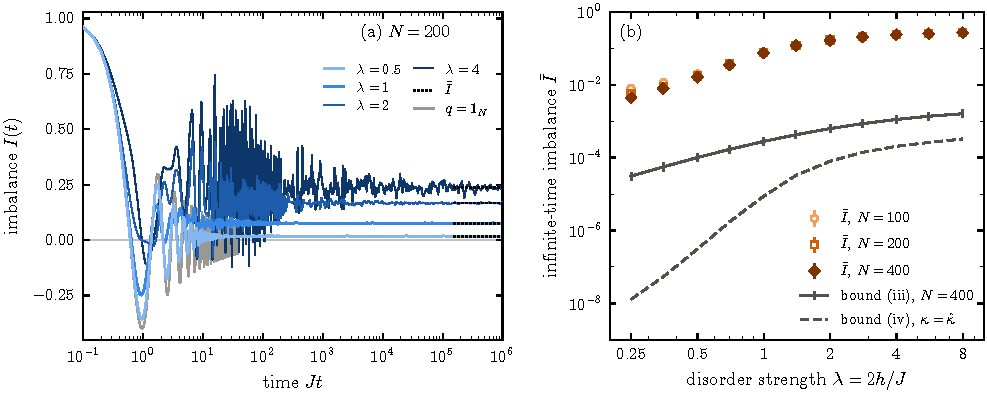
\includegraphics[width=\textwidth]{figs/imbalance.pdf}
\caption{Memory of the charge-density wave, for $\Psi_0=\ket{\uparrow\cdots\uparrow}_z\otimes\psicdw$ and $J=1$.
(a) Imbalance $I(t)$ for $N=200$ and $\lambda=2h/J=0.5,1,2,4$ (light to dark), averaged over the same $1000$
i.i.d.\ charge sectors at all times; uniform time grid for $Jt\le200$, logarithmic grid beyond.  The bands of
$\pm2$ standard errors are mostly thinner than the lines.  The short dotted segments at the right mark the
infinite-time average $\Ibar$ of \cref{thm:imbalance}(i), computed from the eigenvectors of the same sectors.
Grey: the clean sector $q=\one_N$ (for any $h$), shown for $Jt\le40$.  (b) $\Ibar$ versus $\lambda$ for
$N=100,200,400$ ($2000$ sectors each; the error bars of $\pm2$ standard errors are smaller than the symbols),
and the rigorous lower bounds of \cref{thm:imbalance} evaluated with the measured $\kappa_N$: the better of the two
bounds \eqref{eq:main-Ibound} at $N=400$ (solid), and the bound \eqref{eq:main-Iuniform} with $\kappa$ replaced by
$\kaphat=\max_N(\kappa_N+2\,\mathrm{SE})$ (dashed).  See \cref{tab:numerics-imbalance}.}
\label{fig:imbalance}
\end{figure}

\begin{table}[t]
\centering
\small
\setlength{\tabcolsep}{3pt}
\begin{tabular}{c|ccc|c|cc|cc}
$\lambda$ & $\Ibar_{100}$ & $\Ibar_{200}$ & $\Ibar_{400}$ & $\kappa_{400}$ & (iii), $N=400$ & (iv), $\kaphat$
 & $\Sigma_1(\Femp)$ & (iv), $2\Sigma_1(\Femp)$\\\hline
$0.25$ & $0.00782(10)$ & $0.00556(5)$ & $0.00433(3)$ & $43.22(3)$ & $3.1\times10^{-5}$ & $1.3\times10^{-8}$ & -- & --\\
$0.5$ & $0.01968(14)$ & $0.01732(9)$ & $0.01596(6)$ & $15.84(3)$ & $1.0\times10^{-4}$ & $3.1\times10^{-7}$ & -- & --\\
$1$ & $0.0788(4)$ & $0.0759(3)$ & $0.0745(2)$ & $4.95(2)$ & $2.8\times10^{-4}$ & $8.7\times10^{-6}$ & $104$ & $5.0\times10^{-9}$\\
$2$ & $0.1710(8)$ & $0.1672(5)$ & $0.1654(4)$ & $2.42(3)$ & $6.3\times10^{-4}$ & $7.9\times10^{-5}$ & $18.9$ & $3.4\times10^{-7}$\\
$4$ & $0.2402(11)$ & $0.2369(8)$ & $0.2362(5)$ & $2.02(2)$ & $1.1\times10^{-3}$ & $2.0\times10^{-4}$ & $10.9$ & $1.8\times10^{-6}$\\
$8$ & $0.2697(12)$ & $0.2669(9)$ & $0.2640(6)$ & $1.90(3)$ & $1.6\times10^{-3}$ & $3.3\times10^{-4}$ & $8.3$ & $4.5\times10^{-6}$
\end{tabular}
\caption{Infinite-time imbalance and the lower bounds of \cref{thm:imbalance} ($J=1$; $2000$ sectors for each
$N$ and $\lambda$).  $\Ibar_N$: measured $\Ibar$.  $\kappa_{400}$: measured $\kappa_N$ of \eqref{eq:main-kappa} at $N=400$.
(iii): the larger of the two bounds \eqref{eq:main-Ibound} at $N=400$, with $\kappa_N$ replaced by
$\kappa_N+2\,\mathrm{SE}$; at this $N$ it is always the global bound $h^2/(N(J+|h|)^2)$.  (iv), $\kaphat$: the right
side of \eqref{eq:main-Iuniform} with $\kappa=\kaphat=\max_{N\in\{100,200,400\}}(\kappa_N+2\,\mathrm{SE})$, which exceeds
$\kappa_{400}$ by at most $0.07$.  The proof
of \cref{thm:imbalance}(iv) uses $\kappa$ only through $\kappa_N\le\kappa$, so this number is a lower bound on $\Ibar$
for each of the three values of $N$; it is not a statement uniform in $N$.  Last two columns:
$\Sigma_1(\Femp)$ for the empirical correlator envelope $\Femp(d)=\max_x\E_qQ^{[1,400]}_q(x,x+d)$, made
non-increasing, and the right side of \eqref{eq:main-Iuniform} with the constant $\kappa=2\Sigma_1(\Femp)$ that the
proof of \cref{thm:imbalance}(iv) uses.  These are omitted for $\lambda\le0.5$, where $\Femp$ has not decayed at
$d=N-1$.}
\label{tab:numerics-imbalance}
\end{table}

\paragraph{Time traces.}  \Cref{fig:imbalance}(a) shows, in our conventions, the observable studied numerically
in \cite{SKKM2017}.  After a transient, the sector-averaged imbalance settles at a positive value.  This value
agrees with the infinite-time average $\Ibar$ computed from the eigenvectors: at $Jt=10^6$ we find
$I=0.0174(7)$, $0.0747(9)$, $0.1694(16)$ and $0.2365(20)$ for $\lambda=0.5,1,2,4$, against $\Ibar=0.0173(1)$,
$0.0760(4)$, $0.1668(8)$ and $0.2376(11)$ from the same sectors.  The clean sector $q=\one_N$, the only sector of
the strictly gauge-invariant subspace $G_j\equiv1$ (\cref{rem:gaussproj}), has no memory.  In infinite volume its
imbalance is $\sum_{m\in\Z}(-1)^mJ_m(2Jt)^2=J_0(4Jt)$, by Neumann's addition theorem for Bessel functions.  For
$N=200$ it differs from $J_0(4Jt)$ by less than $5\times10^{-3}$ for $Jt\le40$, and its time average vanishes
exactly (\cref{rem:gaussproj}(ii)).  The memory is produced by the sector average, through the mechanism in the
proof of \cref{thm:imbalance}(iii).

\begin{remark}[Slow, oscillatory relaxation at strong coupling; heuristic]\label{rem:num-oscillations}
For $\lambda\ge2$ the approach of $I(t)$ to $\Ibar$ is slow and oscillatory, with deviations far larger than the
statistical errors.  At $\lambda=4$, $I(t)$ oscillates between $-0.12$ and $0.75$ for $Jt\in[10,100]$, and
$I=0.134(2)$ at $Jt=100$ and $0.336(2)$ at $Jt=2.2\times10^3$.  For $Jt\in[10^4,10^6]$ it still deviates from
$\Ibar=0.2376(11)$ by up to $0.06$ ($26$ standard errors).  At $\lambda=2$ the deviations stay below $0.007$
($4$ standard errors) for $Jt\ge10^4$.  For $\lambda\le1$ the data for $Jt\ge10^3$ agree with $\Ibar$ to within
$2.7$ standard errors.

We attribute the slow oscillations to the binary nature of the disorder.  Consider two equal charges at odd
distance $k$, separated by $k-1$ opposite charges.  Their sites are resonant, and the particle that the CDW places
on one of them tunnels to the other through an effective hopping of order $J(2\lambda)^{-(k-1)}$.  This hopping
depends only on the local charge pattern, which takes finitely many values.  The resulting oscillations, at
frequencies $\omega_k\approx2J(2\lambda)^{-(k-1)}$, are therefore coherent across sectors and dephase only through
higher-order, environment-dependent corrections.  For $k=1$ (adjacent equal charges), $\omega_1\approx2J$ gives the
fast oscillations at early times.  Consistently, at $\lambda=4$ ($N=200$, $400$ sectors) the spectral weight of
$I_q(t)-\Ibar_q$ has sharp peaks at $\omega\approx0.030J$, $4.5\times10^{-4}J$ and $6.8\times10^{-6}J$, close to
$\omega_3$, $\omega_5$, $\omega_7=0.031J$, $4.9\times10^{-4}J$, $7.6\times10^{-6}J$.  These correspond to periods of
about $2\times10^2$, $1.3\times10^4$ and $8\times10^5$ in units of $1/J$.  The windows within a factor $1.2$ of $\omega_3$
and $\omega_5$ carry about half of the weight of their decades ($0.022$ of $0.047$, and $0.0029$ of $0.0061$;
\texttt{code/numerics\_imbalance\_spectral.out}).  This explanation is heuristic.  None of it affects $\Ibar$,
which is what \cref{thm:imbalance} controls.
\end{remark}

\paragraph{Infinite-time imbalance.}  \Cref{fig:imbalance}(b) and \cref{tab:numerics-imbalance} show that $\Ibar>0$
at every $\lambda$ considered, down to $\lambda=0.25$, and that $\Ibar$ increases with $\lambda$.  For $\lambda\ge1$ it
decreases by $2$--$6\%$ from $N=100$ to $N=400$.  A boundary correction describes this well: a fit
$\Ibar_N=\Ibar_\infty+c/N$ to the three values has $\chi^2\le2.2$ (one degree of freedom) and $c$ between $0.5$ and
$1.1$ for every $\lambda\ge1$; at $\lambda=2$, for instance, $\Ibar_\infty=0.1635(6)$.  For $\lambda\le0.5$ the convergence in $N$ is slow, as expected when the localization
length is comparable with $N$: $\Ibar=0.01968(14)$, $0.01732(9)$, $0.01596(6)$ at $\lambda=0.5$, and
$0.00782(10)$, $0.00556(5)$, $0.00433(3)$ at $\lambda=0.25$, for $N=100,200,400$.  \Cref{thm:imbalance}(iv) asserts a
positive lower bound uniform in $N$ for every $\lambda\neq0$.  At $\lambda\le0.5$ the data are compatible with it but
cannot test the uniformity: they only show that $\Ibar$ is positive and not yet converged at $N=400$.

\paragraph{The rigorous bounds.}  For $\lambda\ge1$ the measured $\kappa_N$ is nearly independent of $N$; for example
it is $4.83(1)$, $4.93(2)$, $4.95(2)$ at $\lambda=1$ and $2.37(1)$, $2.41(3)$, $2.42(3)$ at $\lambda=2$, for
$N=100,200,400$.  This agrees with the bound $\kappa_N\le\kappa$ of \cref{thm:imbalance}(iv).  For $\lambda\le0.5$ it still
grows with $N$ ($11.25(2)$, $14.27(3)$, $15.84(3)$ at $\lambda=0.5$).  All bounds lie below the data, as they must,
but by large factors.
\begin{itemize}
\item At $N=400$ the better of the bounds \eqref{eq:main-Ibound} is the global one, $h^2/(N(J+|h|)^2)$, which is
$140$--$280$ times smaller than $\Ibar$.  The block bound does not decay with $N$, but its optimal block length
$L\approx32\kappa_N^2$ exceeds $400$ for $\lambda\le1$.
\item The bound \eqref{eq:main-Iuniform}, evaluated with the measured $\kaphat$, is smaller than $\Ibar$ by factors
from $8\times10^2$ (at $\lambda=8$) to $3\times10^5$ (at $\lambda=0.25$).
\item With the constant $\kappa=2\Sigma_1(F)$ that the proof of \cref{thm:imbalance}(iv) uses, evaluated with the
empirical envelope $\Femp$, the bound drops by a further factor between $70$ (at $\lambda=8$) and $1.7\times10^3$
(at $\lambda=1$).
\end{itemize}
The losses have three sources.  The Cauchy--Schwarz step (Step~2 in the proof of \cref{thm:imbalance}) bounds
$\sum_\alpha a_\alpha^2m_\alpha(B)$ below by $X_B^2$ divided by $\sum_\alpha E_\alpha^2m_\alpha(B)\le4L(J+|h|)^2$, which is far
from equality.  In the anticoncentration step (Step~4), Szarek's constant $\sqrt{L/2}$ has to beat the leakage
$2\kappa_N$; this requires $L>8\kappa_N^2$, and the optimal $L$ is of order $32\kappa_N^2$.  Finally, $\kappa_N\le2\Sigma_1(F)$ replaces the time-averaged
probabilities $R_q$ by the correlator $Q_q$ and its envelope.  The content of \cref{thm:imbalance} is qualitative:
a positive memory, uniformly in $N$, for every $h\neq0$.  This is what the data show.

% ----------------------------------------------------------------------------
\subsection{Entanglement and number entropy}\label{sec:numerics:entropies}

\begin{figure}[t]
\centering
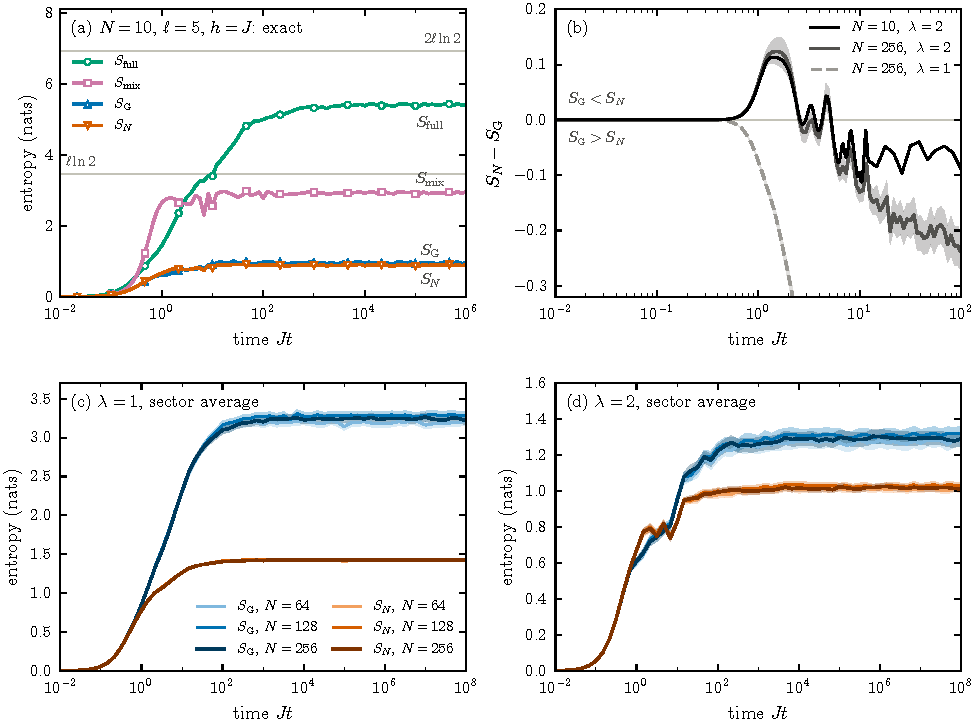
\includegraphics[width=\textwidth]{figs/entropies.pdf}
\caption{Entropies of the half chain after the quench from $\ket{\uparrow\cdots\uparrow}_z\otimes\psicdw$, $J=1$.
(a) Exact values for $N=10$, $\ell=5$, $h=J$ ($\lambda=2$), from the many-body state of the gauge theory (all $1024$
sectors, no sampling): the matter-plus-gauge entanglement $\Sfull$, the mixed dressed-matter entropy $\Smix$, the
conditional entanglement $\SG$ and the number entropy $\SN$.  Grey lines: the maxima $2\ell\ln2$ of $\Sfull$ and
$\ell\ln2$ of $\Smix$.  (b) $\SN-\SG$ at early times, for $N=10$ (exact; black) and for $N=256$ at $\lambda=2$ (dark grey) and $\lambda=1$
(grey, dashed), with $400$ sectors on a grid of $30$ times per decade and bands of $\pm2$ standard errors.  Positive values are counterexamples to the
inequality $\SG\ge\SN$ (\cref{rem:main-SGSN}).  (c), (d) The sector-averaged $\SG(t)$ (blue) and the number entropy
$\SN(t)$ of the mixture (vermillion), for $N=64,128,256$ (light to dark; $1000$ sectors each, bands of $\pm2$
standard errors), up to $Jt=10^8$, at $\lambda=1$ and $\lambda=2$.}
\label{fig:entropies}
\end{figure}

\paragraph{Exact data for $N=10$.}  \Cref{fig:entropies}(a) extends the table of \cref{rem:main-SGSN} to a dense
time grid ($97$ times in $[10^{-2},10^6]$).  The conditional entanglement $\SG$ is $0.91$ at $Jt=10$, and for
$Jt\in[10^3,10^6]$ it stays in $[0.93,0.99]$.  The full entanglement keeps growing over several decades, from
$\Sfull=1.45$ at $Jt=1$ to $3.40$, $5.00$ and $5.38$ at $Jt=10$, $10^2$ and $10^5$.  For $Jt\in[10^3,10^6]$ it stays in
$[5.30,5.45]$, below the maximum $2\ell\ln2=6.93$.  This is consistent with the logarithmic growth of
Conjecture~\ref{conj:logent} followed by finite-size saturation, but $N=10$ cannot separate the two.  The mixed
entropies saturate near $0.85\,\ell\ln2$: for $Jt\ge10^3$, $\Smix\in[2.89,2.97]$ and $\Sfm\in[2.92,3.00]$
(cf.\ Conjecture~\ref{conj:volmix}).  The number entropy stays in $[0.87,0.92]$.  The inequalities of
\cref{prop:entropies} hold at all $97$ times: $|\Sfull-S_{A'}(\Phi)|\le0.56<\ln2$, $\SG\le\Smix\le\ell\ln2$,
$\SN\le\min\{\Sfull,\Smix,\Sfm\}$ and $\E_q\Hsh(p^q_t)\le\min\{\SG,\SN\}$.

\paragraph{$\SG$ versus $\SN$.}  \Cref{fig:entropies}(b) shows where the false inequality $\SG\ge\SN$ fails.  For
$N=10$ (computed on a grid of step $0.005$ in $[0.05,12]$), $\SN-\SG>0$ for $0.05\le Jt<2.575$, with maximum $0.113$ at
$Jt\approx1.4$.  The difference then changes sign five times, at $Jt\approx2.58$, $2.93$, $3.63$, $4.25$ and $5.23$,
staying below $0.044$ in modulus, and $\SG>\SN$ at all later grid times up to $Jt=10^6$.  The same happens in large systems at $\lambda=2$.  For $N=256$
($400$ sectors, $30$ times per decade), $\SN-\SG$ exceeds two standard errors at all grid times
$0.015\le Jt\le2.33$, with maximum $0.124(11)$ at $Jt\approx1.5$.  On our grid it changes sign five times between
$Jt\approx2.5$ and $Jt\approx5.4$, staying below $0.044$ in modulus, and it is below minus two standard errors at all grid times
$5.4\le Jt\le10^2$.  At $\lambda=1$ (again $N=256$) the difference never exceeds
$2\times10^{-10}$, and it is below minus two standard errors for $Jt\ge0.074$.  Heuristically, the mechanism is the
one described in \cref{rem:main-SGSN}.  At early times about one particle crosses the cut, each $\rho^q_A$ is close to
a mixture of two number sectors, and so $\SG\approx\E_q\Hsh(p^q_t)\le\Hsh(\E_qp^q_t)=\SN$, by concavity.  The gap $\Hsh(\E_qp^q_t)-\E_q\Hsh(p^q_t)$ is the mutual information between $N_A$ and the charges, and it
grows with the spread of the per-sector laws.  At $Jt=1$ and $N=256$, the variance of the sector means
$\langle N_A\rangle_q$ (that is, $\Var_{p_t}(N_A)-\E_q\Var_q(N_A)$) is $0.039$ at $\lambda=2$ and $0.0053$ at $\lambda=1$; two
independent samples of $1000$ and $400$ sectors agree on these values to $3\%$.

\paragraph{Large $N$.}  \Cref{fig:entropies}(c), (d) show $\SG$ and $\SN$ for $N=64,128,256$ up to $Jt=10^8$.  Both
saturate after $Jt\approx10^2$--$10^3$.  They then stay flat: for every $N$ and both values of $\lambda$, the averages over
the grid times in $[10^3,10^5]$ and in $[10^6,10^8]$ differ by less than $0.01$, which is within the errors.  There is
no sign of the slow growth seen in $\Sfull$.  Averaging over the grid times $Jt\ge10^3$, with errors over sectors,
we find for $N=64,128,256$:
\begin{center}
\begin{tabular}{c|ccc|ccc}
 & \multicolumn{3}{c|}{$\SG$} & \multicolumn{3}{c}{$\SN$}\\
 & $N=64$ & $N=128$ & $N=256$ & $N=64$ & $N=128$ & $N=256$\\\hline
$\lambda=1$ & $3.19(2)$ & $3.28(2)$ & $3.24(2)$ & $1.420(4)$ & $1.431(4)$ & $1.425(4)$\\
$\lambda=2$ & $1.27(2)$ & $1.31(2)$ & $1.29(2)$ & $1.011(7)$ & $1.028(7)$ & $1.016(8)$
\end{tabular}
\end{center}
The values for different $N$ agree to within $3\%$.  The largest difference, $2.9$ standard errors, is between $N=64$
and $N=128$ for $\SG$ at $\lambda=1$, and the value for $N=256$ lies between the two.  This is what
\cref{thm:arealaw}(b) and \cref{thm:numberentropy} assert: both entropies are bounded uniformly in $t$ and $N$.  The
quantity bounded in \cref{thm:arealaw}(b) is $\E_q\sup_tS(\rho^q_A(t))$.  Its lower estimate
$\E_q\max_{t\in\mathcal T}S(\rho^q_A(t))$ over our time grid $\mathcal T$ is $3.92(3)$, $4.02(3)$, $3.96(3)$ at
$\lambda=1$ and $1.68(2)$, $1.74(2)$, $1.71(2)$ at $\lambda=2$, for $N=64,128,256$.

\paragraph{Size of the constants.}  The theorems hold with the true function $F$ of Hypothesis~\ref{hyp:EC}, whose
constants are not explicit (\cref{rem:rate}).  To indicate their size we insert the empirical envelope $\Femp$ of
\cref{tab:numerics-imbalance} ($N=400$).  At $\lambda=2$ this gives $2\ln2\,\Theta(\Femp)\approx1.3\times10^3$ for the
area-law bound of \cref{thm:arealaw}(b), against a measured $\E_q\max_{t\in\mathcal T}S(\rho^q_A(t))\approx1.7$.  It gives
$\frac12\ln(2\pi e(K_1+K_2+\frac1{12}))\approx6.3$ for the bound \eqref{eq:main-SN}, against a measured $\SN\approx1.0$.
At $\lambda=1$ the two bounds are $1.5\times10^4$ and $7.8$, against $4.0$ and $1.4$.  The number-entropy bound is much
closer to the data only because the constants enter it through a logarithm.  Inserting the \emph{measured} variance of
$N_A$ into \cref{lem:intentropy} gives $1.11$--$1.13$ at $\lambda=2$ and $1.47$--$1.48$ at $\lambda=1$ (maximum over $t$),
close to the measured $\SN$.  This uses the measured variance instead of the bound $K_1+K_2$, so it is not a consequence
of \cref{thm:numberentropy} (\cref{rem:main-numberentropy}).

% ----------------------------------------------------------------------------
\subsection{One-body localization and the dimer law}\label{sec:numerics:other}

Two further figures appear in the sections they illustrate.

\Cref{fig:correlator} (\cref{sec:onebody}) shows the annealed eigenfunction correlator $\E_qQ^{[1,N]}_q(x,x+d)$, the
quantity of Hypothesis~\ref{hyp:EC}, for boundary pairs ($x=1$) and bulk pairs ($x=N/2$) and $N=100,200,400$.  The
boundary and bulk correlators decay at the same rate and do not depend on $N$.  This is the content of
\cref{thm:EC}: uniformity in $N$ and in the position of the pair, including pairs at the fixed left end of the chain.
The fitted annealed rates reported in \cref{rem:onebodynumerics} lie well below the smallest Lyapunov exponent,
increasingly so as $\lambda$ grows, in line with \cref{rem:rate}(ii).

\Cref{fig:dimer} (\cref{sec:dimer}) shows one dressed fermion in a dimer product state, for which the sector law is the
random dimer law (\cref{prop:dimerlaw}).  At $h=0.25J$, where $0<2h<J$ and the dimer model has critical energies, the
sector-averaged mean-square displacement grows superdiffusively, roughly like $t^{3/2}$.  The time-averaged moment
$\Mom_2(T)$ of every sampled sector is bounded below by a multiple of $JT$, as \cref{prop:dimerlower} and
\cref{thm:dimer} assert.  For the i.i.d.\ law at the same $h$, and for the dimer law at $h=0.75J$, the mean-square displacement
saturates (\cref{rem:dimernumerics}).  The Hamiltonian is the same in all these runs; only the initial state differs, and with
it the sector law.  Together with \cref{fig:imbalance}, this illustrates that disorder-free localization is a
property of the sector law induced by the initial state (\cref{rem:dimermessage}).

% ----------------------------------------------------------------------------
\subsection{What the numerics do and do not show}\label{sec:numerics:summary}

\begin{remark}[Scope]\label{rem:num-scope}
(i) All data are for finite $N$ and finite times, and the sector averages for $N\ge64$ are Monte Carlo estimates
with the quoted errors.  They illustrate the theorems.  They cannot confirm statements about $N\to\infty$ or
$t\to\infty$, and they are not used in any proof.

(ii) Every rigorous bound that we evaluated holds in the data, and none is close to sharp.  With the measured
$\kappa_N$, the lower bounds on $\Ibar$ are $10^2$ to $3\times10^5$ times too small, and up to $1.5\times10^7$ times with
the constant of \cref{thm:imbalance}(iv) evaluated with $\Femp$.  Evaluated with $\Femp$, the area-law bound exceeds the
measured $\E_q\max_{t\in\mathcal T}S(\rho^q_A(t))$ by factors of about $8\times10^2$ ($\lambda=2$) and $4\times10^3$
($\lambda=1$), and the number-entropy bound exceeds the measured $\SN$ by factors of $5$--$6$.

(iii) The exact $N=10$ data are consistent with Conjectures~\ref{conj:logent} and~\ref{conj:volmix}, but they do
not test them.  A test would need the full many-body state of much larger systems.
\end{remark}
